\documentclass[a6paper,landscape]{scrartcl}
\usepackage[margin=0.4cm,bottom=0cm]{geometry}
\usepackage{tikz}
\usepackage[utf8]{inputenc}


\input{code128.tex}

\barheight=0.5cm
\newcommand{\myhrule}{\rule[3pt]{7pt}{1pt}}
\newcommand{\myhrulefill}{\leaders \hbox{\rule[3pt]{1pt}{1pt}} \hfill}
\usetikzlibrary{patterns}
\tikzset{%
	block/.style={draw,fill=blue!30,minimum height=3em,%
		minimum width=10em,line width=0.5pt,inner xsep=0.7em},
	aussen/.style={inner sep=0pt}}

\begin{document}
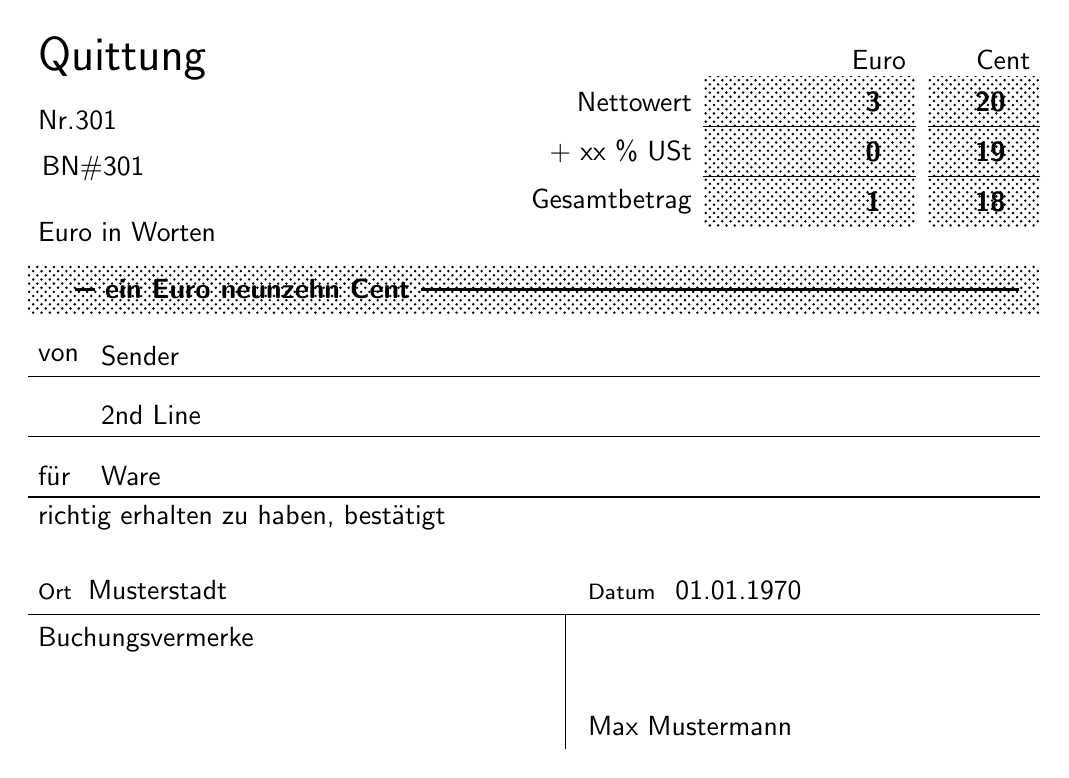
\begin{tikzpicture}[%
x=1cm,y=1cm,font=\sffamily]

\node[anchor=east] at (13.970, 22.75) {Euro};
\node[anchor=east] at (15.55, 22.75) {Cent};

\node[anchor=east] at (11.25 , 22.225) {Nettowert};
\node[anchor=east] at (11.25, 21.59) {+ xx \% USt};
\node[anchor=east] at (11.25, 20.955) {Gesamtbetrag};

% Nettobetrag Cent
\fill[pattern=crosshatch dots] (14.129, 22.543) rectangle (15.55, 21.907);
% USt Cent
\fill[pattern=crosshatch dots] (14.129, 21.907) rectangle (15.55, 21.273);
% Gesamtbetrag Cent
\fill[pattern=crosshatch dots] (14.129, 21.273) rectangle (15.55, 20.637);

%TODO Possible Replacement
\draw[anchor=south west] (15.55,21.273) -- (14.129,21.273);
\draw[anchor=south west] (14.129, 21.907) -- (15.55, 21.907);

%Netto Cent
\fill[pattern=crosshatch dots] (11.271, 22.543) rectangle (13.970, 21.907);
%USt Cent
\fill[pattern=crosshatch dots] (11.271, 21.907) rectangle (13.970, 21.273);
% Gesamtbetrag Euro
\fill[pattern=crosshatch dots] (11.271, 21.273) rectangle (13.970, 20.637);

\fill[pattern=crosshatch dots] (2.699, 20.161) rectangle (15.55, 19.526);



%TODO Possible Replacement
\draw[anchor=south west] (11.271, 21.273) -- (13.970, 21.273);
\draw[anchor=south west] (13.970, 21.907) -- (11.271, 21.907);

%Constuction Bottom
%TODO Cleanup
\draw[anchor=south west] (9.525, 14) -- (9.525, 15.716);
\draw[anchor=south west] (2.699, 15.716) -- (15.55, 15.716);

\draw[anchor=south west] (2.699, 17.977) -- (15.55, 17.977);

\draw[anchor=south west] (2.699, 17.204) to (15.55, 17.204);
\draw[anchor=south west] (2.699, 18.733) to (15.55, 18.733);

\node[anchor=west] at (2.699, 15.399) {Buchungsvermerke};
\node[anchor=south west] at (2.699, 15.783) {\footnotesize{Ort}};

\node[anchor=west] at (2.699, 16.937) {richtig erhalten zu haben, bestätigt};

\node[anchor=west] at (2.699, 17.471) {für};

\node[anchor=west] at (2.699, 19) {von};

\node[anchor=south west] at (2.699, 20.320) {Euro in Worten};

\node[anchor=south west] at (2.699, 22.384) {\LARGE{Quittung}};

\node[anchor=south west] at (2.699, 21.749) {Nr.};

\node[anchor=west] at (3.5, 19) {Sender};

\node[anchor=south west] at (3.175, 21.749) {301};
\node[anchor=south west] at(2.749, 21.1) {\code{BN\#301}};

%
% Fig TEXT object
%
\node[anchor=west] at (3.175, 19.8435) {\textbf{\makebox[12cm]{\myhrule{ ein Euro neunzehn Cent }\myhrulefill}}};
%
% Fig TEXT object
%
\node[anchor=west] at (3.5, 17.471) {Ware};
%
% Fig TEXT object
%
\node[anchor=south west] at (9.684, 14.05){Max Mustermann};
%
% Fig TEXT object
%
\node[anchor=south west] at (9.684, 15.783) {\footnotesize{Datum}};
%
% Fig TEXT object
%
\node[anchor=south west] at (3.334, 15.783) {Musterstadt};
%
% Fig TEXT object
%
\node[anchor=south west] at (10.795, 15.783) {01.01.1970};
%
% Fig TEXT object
%
\node[anchor=west] at (3.5, 18.244){2nd Line};
%
% Fig TEXT object
%
\node[anchor=east] at (13.652, 22.225){\textbf{3}};
%
% Fig TEXT object
%
\node[anchor=east] at (13.652, 21.59) {\textbf{0}};
%
% Fig TEXT object
%
\node[anchor=east] at (13.652, 20.955) {\textbf{1}};

\node[anchor=west] at (14.60,22.225) {\textbf{20}};
\node[anchor=west] at (14.60, 21.59) {\textbf{19}};
\node[anchor=west] at (14.60, 20.955) {\textbf{18}};


\end{tikzpicture}

\end{document}